 \begin{figure*}
 \centering
 % 115 classes
 \begin{minipage}[t]{0.45\linewidth}
 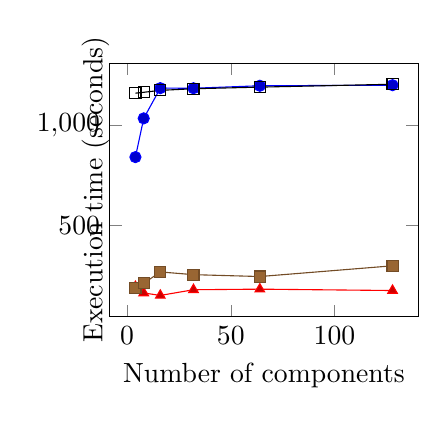
\begin{tikzpicture}
 \begin{axis}[
 	ylabel={Execution time (seconds)},
 	y label style={at={(0.03, 0.5)}},
 	xlabel={Number of components},width = 5.5cm,
 	height = 4.8cm]

 \addplot+[mark=*] coordinates
 	{(4,842.274) (8,1035.734) (16,1186.657) (32,1186.140) (64,1198.539) (128,1201.415)};
 	
 \addplot+[mark=triangle*] coordinates
 	{(4,195.609) (8,163.964) (16,151.637) (32,180.026) (64,182.962) (128,176.101)};
 	
 \addplot+[mark=square*] coordinates
	 	{(4,186.798) (8,211.913) (16,268.908) (32,255.329)  (64,245.976) (128,299.516)};
	 	
 \addplot+[mark=square] coordinates
	 	{(4,1161.593) (8,1165.910) (16,1175.643) (32,1183.620)  (64,1191.749) (128,1206.128)};
 \end{axis}
 \end{tikzpicture}
 \caption{Execution time of main task with\newline a component size of 115 classes.\label{fig:execution-time-many-115}}
\end{minipage}
 % 4 classes
 \begin{minipage}[t]{0.45\linewidth}
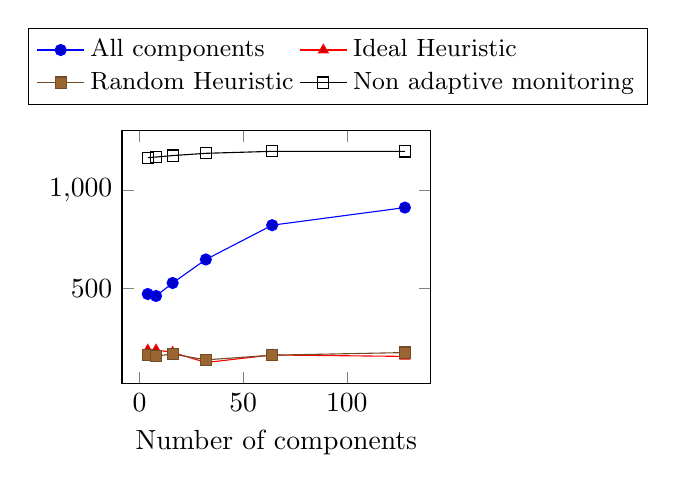
\begin{tikzpicture}
 \begin{axis}[
 	every axis legend/.append style={nodes={right}},
 	legend columns=2,
 	legend style={at={(0.7,1.1)},
 	anchor=south,legend columns=1, font=\small},
 	xlabel={Number of components},width = 5.5cm,
 	height = 4.8cm]

\addplot+[mark=*] coordinates
 	{(4,471.532) (8,461.274) (16,527.667) (32,647.634) (64,822.767) (128,912.634)};
 	
 \addplot+[mark=triangle*] coordinates
 	{(4,185.003) (8,185.533) (16,173.457) (32,121.551) (64,160.201) (128,152.802)};
 	
 \addplot+[mark=square*] coordinates
	 	{(4,161.985) (8,154.983) (16,164.704) (32,135.131)  (64,159.032) (128,172.392)};
	 	
 \addplot+[mark=square] coordinates
	 	{(4,1167.814) (8,1170.811) (16,1178.219) (32,1189.748)  (64,1199.834) (128,1199.453)};

	\legend{All components, Ideal Heuristic, Random Heuristic, Non adaptive monitoring}
 \end{axis}
 \end{tikzpicture}
 \caption{Execution time of main task with\newline a component size of four classes.\label{fig:execution-time-many-4}}
 \end{minipage}
\hspace{1.5cm}
\end{figure*}
